\chapter{Experiment 2: Partial grouping in one frame}

\section{Introduction}
To evaluate whether the grouping of partials with common AM and FM parameters is
plausible, we synthesize a set of parameters and test by corrupting the
parameters with noise and adding spurious sets of parameters that should not
belong to any sources.

\section{Methodology}
We assume parameters have been estimated already so we start from theoretical
values for the amplitude, frequency, frequency modulation and amplitude
modulation.  On each frame of analysis data, i.e., for parameters belonging to
the same time instant, we consider each data-point as a multi-dimensional random
variable. With these random variables, we compute principal components in order
to produce a variable with maximum variance. This variable is classified using a
clustering algorithm and we evalutate the results. A summary follows:
\begin{itemize}
    \item 
        Parameters are synthesized from a theoretical mixture of AM and FM
        sinusoids.  Spurious data are added to these parameters.
    \item
        Principal components analysis is carried out on the parameters happening
        at one time instance.
    \item
        A histogram is made of the 1st principal components. Values sharing a
        bin with too few other values are discarded to remove spurious data
        points.
    \item
        Initial means and standard deviations for the Gaussian mixture models
        are made by dividing the histogram into equal parts by area and choosing
        the centres of these parts.
    \item
        The EM algorithm for Gaussian mixture models is carried out to classify
        the sources.
\end{itemize}
\section{Evaluation}
The algorithm is run on a typical source separation problem to evaluate its
plausibility.
\section{Synthesis}
Our model makes available the following parameters. Time values are in seconds,
frequency values are in $Hz$ and phase values are in radians.
\begin{itemize}
    \item
        $t$ time.
    \item
        $f_{s}$ sampling frequency.
    \item
        $N$ length of signal in samples.
    \item
        $H$ duration between data-point calculations in samples (i.e., the hop
        size).
    \item
        $N_{p}$ number of sources.
    \item
        $p$ which source.
    \item
        $f_{0,p}$ fundamental frequency.
    \item
        $K_{p}$ number of harmonics.
    \item
        $k_{60,p}$ harmonic number 60 dB lower than the first.
    \item 
        $B_{p}$ the inharmonicity coefficient.
    \item
        $\phi_{0,p}$ initial phase.
    \item
        $\phi_{0,f,p}$ initial FM phase.
    \item
        $t_{60,p}$ time until amplitude of partial has dropped 60 dB.
    \item
        $t_{\text{attack},p}$ time duration of attack portion.
    \item
        $A_{f,p}$ amplitude of FM.
    \item
        $f_{f,p}$ frequency of FM.
    \item
        $s_{p}$ the signal representing the $p$th source.
\end{itemize}

To incorporate inharmonicity often observed in real string instruments where the
strings exhibit some stiffness, we define the \textit{stretched} harmonic numbers
as follows
\cite{paspweb2010}\footnote{
\texttt{http://ccrma.stanford.edu/\~{}jos/pasp/Dispersion\_Filter\_Design\_I.html}}

\begin{equation}
    K_{B}(k) = k (1+Bk^{2})^{\frac{1}{2}}
\end{equation}

Each source is synthesized using the following equation:
\begin{equation}
    s_{p}(t) = \sum_{k=1}^{K_{p}} A_{p}(k,t) \exp(j(2\pi
    f_{0,p}t - \frac{A_{f,p}}{f_{f,p}} \cos(2\pi f_{f,p} t +
    \phi_{0,f,p}) K_{B_{p}}(k) + \phi_{0,p}))
\end{equation}
where
\begin{equation}
    A_{p}(k,t) = 
    \begin{cases}
        \exp(a_{60,p} t + a_{k,60,p}k) \cos^{2}
        (\frac{\pi}{2}(\frac{t}{t_{\text{attack},p}} - 1)) & \text{if } t \leq
        t_{\text{attack},p},\\
        \exp(a_{60,p} t + a_{k,60,p}k) & \text{if } t > t_{\text{attack},p},\\
        0 & \text{otherwise}.
    \end{cases}
\end{equation}
\begin{equation}
    a_{60,p} = \frac{\log(10^{-3})}{t_{60,p}}
\end{equation}
\begin{equation}
    a_{k,60,p} = \frac{\log(10^{-3})}{k_{60,p}} 
\end{equation}
The piecewise amplitude function is based on the amplitude function of the
\textit{Formant Wave Function (FOF)}\footnote{FOF stands for \textit{Forme
d'Onde Formantique}.} described in \cite[p.~19]{rodet1984chant}.

The estimation of these parameters is a separate problem addressed by the
DDM (see Section~\ref{sec:ddm_description}). We use theoretical values calculated
directly from the model signals. For interpretation, and to make it possible to
simply replace the theoretical values with those obtained from an analysis, we
compute parameters that correspond to the model of these methods.

The DDM seeks signals $s_k \in \mathbb{C}$ of the following form:
\begin{equation}
    s_{k}(n) = \exp(\log(A_{k} + \mu_{k}n + j(\phi_{k} + \omega_{k}n +
    \frac{1}{2} \psi_{k} n^{2}))) \label{eq:rm_model}
\end{equation}
Here $n$ is the sample number. Typically when performing a short-time analysis,
the time corresponding to $n = 0$ is made to be the centre of the window,
therefore, $t$ is the time at the centre of the window and $N_{w}$, in samples,
is the length of the middle (usually non-zero) portion of the window. The
coefficents of the $k$th harmonic of the $p$th source from our synthetic model
are given by
\begin{equation}
    \mu_{k,p}(t) = \frac{a_{60,p}}{f_{s}}
\end{equation}
\begin{equation}
    A_{k,p}(t) = \exp(a_{60,p} t + a_{k,60,p} k)
\end{equation}
for the part of the signal after the attack portion.

For the attack portion, we estimate the parameters using least-squares on a
rectangular-windowed signal. Let
\begin{equation}
    \hat{\mathbf{s}}(t) =
    \begin{pmatrix}
        \exp \left(\displaystyle a_{60,p} \left( t - \frac{N_{w}}{2f_{s}} \right)  +
        a_{k,60,p} k \right) \cos^{2} \left(\displaystyle \frac{\pi}{2} \left(
                \frac{ t
        - \frac{N_{w}}{2f_{s}} }{ t_{\text{attack},p}} - 1 \right) \right)  \\
        \vdots \\
        \exp \left(\displaystyle a_{60,p} \left( t + \frac{N_{w}}{2f_{s}} \right)  +
        a_{k,60,p} k \right) \cos^{2} \left(\displaystyle \frac{\pi}{2} \left(
                \frac{ t
        + \frac{N_{w}}{2f_{s}}  }{ t_{\text{attack},p}} - 1 \right) \right)
    \end{pmatrix}
\end{equation}
then $\log(A_{k,p})$ and $\mu_{k,p}$ are found as the least-squares solution of
\begin{equation}
    \begin{bmatrix}
        1 & \frac{-N_{w}}{2} \\
        \vdots & \vdots \\
        1 & \frac{N_{w}}{2}
    \end{bmatrix}
    \begin{pmatrix}
        \log(A_{k,p}(t)) \\
        \mu_{k,p}(t)
    \end{pmatrix}
    = \log{\hat{\mathbf{s}}(t)}
\end{equation}

for the argument parameters (those multiplied by $j$ in Equation~\eqref{eq:rm_model})

\begin{equation}
    \omega_{k,p} \left( t \right)  = \frac{2 \pi}{f_{s}}  \left(  f_{0,p} +
    A_{f,p} \sin \left( 2 \pi f_{f,p} t + \phi_{0,f,p} \right)  \right)
    K_{B_{p}} \left( k \right) 
\end{equation}
\begin{equation}
    \psi_{k,p} \left( t \right)  =  \left( \frac{2 \pi}{f_{s}} \right) ^{2}
    A_{f,p} f_{f,p}  \left(  f_{0,p} + A_{f,p} \cos \left( 2 \pi f_{f,p} t +
    \phi_{0,f,p} \right)  \right)  K_{B_{p}} \left( k \right) 
\end{equation}
\begin{equation}
    \phi_{k} \left( t \right)  =  \left( 2\pi f_{0,p}t - \frac{A_{f,p}}{f_{f,p}}
    \cos \left( 2\pi f_{f,p} t + \phi_{0,f,p} \right)  \right)  K_{B_{p}} \left(
    k \right)  + \phi_{0,p}
\end{equation}

To simulate the noise that would be present in an estimation of the signal
parameters from an arbitrary signal, we create noise corrupted values by
substituting the random variables:
\begin{itemize}
    \item
        $\tilde{\Psi}_{k,p}(t) \sim
        \mathcal{N}(\psi_{k,p}(t),\psi_{no})$
    \item
        $\tilde{\Omega}_{k,p}(t) \sim
        \mathcal{N}(\omega_{k,p}(t),\omega_{no})$
    \item
        $\tilde{\mu}_{k,p}(t) \sim
        \mathcal{N}(\mu_{k,p}(t),\mu_{no})$
    \item
        $\tilde{A}_{k,p}(t) \sim
        \mathcal{N}(A_{k,p}(t),A_{no})$
\end{itemize}
%% If using correlated random variables
%\begin{itemize}
%    \item
%        $\tilde{\Psi}_{k,p}(t) \sim
%        \mathcal{N}(\psi_{k,p}(t),\psi_{no})$
%    \item
%        $\tilde{\Omega}_{k,p}(t) \sim
%        \mathcal{N}(\omega_{k,p}(t),\omega_{no})
%        + \tilde{\psi}_{k,p}(t-\Delta t) \Delta t)$
%    \item
%        $\tilde{\Phi}_{k,p}(t) =
%        \tilde{\omega}_{k,p}(t - \Delta t) \Delta t$
%    \item
%        $\tilde{\mu}_{k,p}(t) \sim
%        \mathcal{N}(\mu_{k,p}(t),\mu_{no})$
%    \item
%        $\tilde{A}_{k,p}(t) \sim
%        \mathcal{N}(A_{k,p}(t),A_{no})$
%\end{itemize}
The $\theta_{no}$ (where $\theta$ is replaced by $\omega$ etc.) specifies the
variance of the particular parameter. Most-likely in practice these random
variables would be correlated but we cannot at this point say anything about
this correlation. Therefore the noisy parameters are uncorrelated random
variables for this experiment.

We also add spurious data-points as a fraction $r_{s}$ of the number of true
data-points. Their values are drawn from uniform distributions with boundaries
$\theta_{s,min}$ and $\theta_{s,max}$, where $\theta$ is some parameter above,
e.g., $\omega_{s,min}$ and $\omega_{s,max}$ for the $\omega$ parameter.

Data points are computed for the times $t = 0,\frac{H}{f_{s}},\frac{2
H}{f_{s}},\ldots,\frac{\left\lfloor \frac{N}{H} \right\rfloor H}{f_{s}}$.

\section{Computation of Principal Components}

At each time $t$ we have $L$ data-points. As the source of each data-point is
now unknown, we replace the $k$ and $p$ indices with index $l$. We only consider
the amplitude and frequency modulation. According to our model, the frequency
modulation is greater for harmonics of greater centre frequency. To take this
into consideration, we divide the frequency modulation estimate $\psi_{l}(t)$ by
the constant frequency estimate $\omega_{l}(t)$ (see thesis by Creager).  The amplitude modulation
$\mu_{l}(t)$ remains constant for all harmonics of the same source, only its initial value
changes according to $k_{60,p}$.  We compile the data-points at one time into a
set of observations
\begin{equation}
    \mathbf{x}_{l}(t) = \begin{pmatrix}
        \frac{\psi_{l}(t)}{\omega_{l}(t)} \\
        \mu_{l}
    \end{pmatrix}
\end{equation}
\begin{equation}
    \mathbf{X}(t) = \begin{bmatrix}
        \mathbf{x}_{1}(t) \ldots \mathbf{x}_{L}(t)
    \end{bmatrix}
\end{equation}
From these $L$ observations the correlation matrix $\mathbf{S}$ is computed. We
use the correlation matrix because the values in each row of $\mathbf{x}_{l}(t)$ do
not have the same units (see Jolliffe for a discussion about this). 

Following the standard technique for producing principal components (see
Jolliffe), we obtain a matrix $\mathbf{V}(t)$ of eigenvectors sorted so that the
eigenvector corresponding to the largest eigenvalue is in the first column, etc.
The principal components $\mathbf{A}(t)$ are then computed as
\begin{equation}
    \mathbf{A}(t) = \mathbf{V}^{T}(t)\mathbf{X}(t)
\end{equation}
We have found it sufficient to use only the first principal component and
therefore only use the values in the first row of $\mathbf{A}(t)$

If we see the $\mathbf{x}_{l}(t)$ as realizations of a random variable, the
above computation of principal components has the effect of projecting
realizations of $\mathbf{x}_{l}(t)$ to points $a_{1,l}(t)$ on a 1-dimensional
subspace. It is a fundamental theory of principal components that the
transformation above maximizes the expected euclidean distance between the
points $a_{1,l}(t)$. This is desirable for the current problem because it will
always produce a variable emphasizing the parameter with the most variance,
hence if we are observing a random variable drawn from multiple distributions
with sufficiently separated means and small enough variances, this separation
will be most observable in the principal components corresponding to the
greatest eigenvalues.

\section{Preparing data for clustering}
The Expectation Maximization underlying the Gaussian mixture model parameter
estimation will only converge to a local maximum (see Dempster et al), therefore, for the best
results, we compute a good initial guess and remove obvious outliers before
carrying out the clustering algorithm.

The $a_{1,l}(t)$ are compiled into a histogram of $N_{b}$ bins. The minimum and
maximum bin boundaries are computed from the maximum and minimum values of
$a_{1,l}(t)$ respectively. Values in a bin with less than $\tau_{h}$ other
values are discarded. We find $N_{p}$ contiguous sections of equal area in the
new histogram omitting the discarded values.  We use the centres of these
sections as the initial mean guesses and half their width as the distance 3
standard deviations from the mean (roughly 99.7 percent of values drawn from one
distribution will lie within this interval if they indeed follow a normal
distribution). The initial guesses for the weights are simply $\frac{1}{N_{p}}$.

\section{Clustering}
Gaussian mixture model parameter estimation will be discussed in an appendix of
this document. After convergence we have an estimated probability
$p(a_{1,l}(t) \text{ from distribution }p)$. We choose the
distribution $p$ for each $a_{1,l}(t)$ that gives the highest probability of it
having occured. The values $\mathbf{x}_{t}(t)$ corresponding to the $a_{1,l}(t)$
have this same classification. Those sharing the same classification can be
interpreted as coming from the same source. The figure shows the results of the
above steps carried out on a mixture of two sources synthesized with the
following parameters:
\begin{table}
    \begin{center}
        \begin{tabular}{c c c }
            Parameter & Source 1 value & Source 2 value \\
            \hline
            $f_{0,p}$ & 261.63 & 277.18 \\
            $K_{p}$ & 20 & 20 \\
            $k_{60,p}$ & 20 & 20 \\
            $B_{p}$ & 0.001 & 0.001 \\
            $\phi_{0,p}$ & 0 & 0 \\
            $\phi_{0,f,p}$ & 0 & 0.8 \\
            $t_{60,p}$ & 0.5 & 0.75 \\
            $t_{\text{attack},p}$ & 0.1 & 0.1 \\
            $A_{f,p}$ & 11.486 & 11.486 \\
            $f_{f,p}$ & 3 & 2
        \end{tabular}
    \end{center}
\end{table}
The length of the signal $N$ is 8000 samples and the anlaysis hop size $H$ is 256
samples.

%\begin{figure}
%    \centering
%\includegraphics[width=\textwidth,height=\textheight]{/home/sandman/Documents/development/masters_thesis/experiment_1/plots/time_frequency_spurious.ps}
%\end{figure}

The data-points are represented as line segments to show the frequency slope.
Data points classified as coming from the same source are dark blue and cyan,
respectively.  Data points classified as spurious are in black. Note that the
classification is done on a frame by frame basis so it could be that data-points
adjacent in time that seem to come from the same source are in different
colours. This is to be addressed in the sequel.
(TODO: how do we choose levels of noise to test against? My current method is to
multiply the value by a random number drawn from a normal distribution + 1. The amount
of change is nicely interpretable as a percentage deviating from the original

